%\documentclass[draft]{article}

\documentclass[pdftex,12pt,letterpaper]{article}
\usepackage[margin=1in]{geometry}
\usepackage[pdftex]{graphicx}
\usepackage{amsmath}
\usepackage[font=footnotesize,labelfont=bf,margin=0.5in,justification=justified, singlelinecheck=on]{caption}
\usepackage{float}

% Allow superscript citations
\usepackage[superscript]{cite}

% Captions
%\usepackage[margin=0.5in,justification=justified, singlelinecheck=on]{caption}
\captionsetup[table]{singlelinecheck=on}

\newcommand{\HRule}{\rule{\linewidth}{0.5mm}}

\begin{document}

% % % % % % % % % % % % % % % % % % % % % % % % % % % % % % % % % % % % % % % %
% % % % % % % % % % % % % % % % % % % % % % % % % % % % % % % % % % % % % % % %
		% 						         Laboration														          %
% % % % % % % % % % % % % % % % % % % % % % % % % % % % % % % % % % % % % % % %
%% % % % % % % % % % % % % % % % % % % % % % % % % % % % % % % % % % % % % % % %

\begin{titlepage}
\begin{center}

% Upper part of the page. The '~' is needed because \\
% only works if a paragraph has started.

\includegraphics[width=0.5\textwidth]{./logo}~\\[1cm]

\vspace{4cm}

\textsc{\Large Biomedical Instrumentation}\\[0.5cm]

% Title
\HRule \\[0.4cm]
{ \huge \bfseries ECG Amplifier Laboration \\[0.4cm] }

\HRule \\[1.5cm]

% Author and supervisor
\noindent
\begin{minipage}{0.4\textwidth}
\begin{flushleft} \large
\emph{Authors:}\\
Courtney \textsc{Keeler} \\
Arsalan \textsc{Latif}
\end{flushleft}
\end{minipage}%
\begin{minipage}{0.4\textwidth}
\begin{flushright} \large
\emph{Professor:} \\
Dr.~Sabine \textsc{Reinfeldt} \\
\emph{TA:} \\
Cristina \textsc{Rigato}
\end{flushright}
\end{minipage}

\vfill

% Bottom of the page
{\large \today}

\end{center}
\end{titlepage}

\section{Introduction}

Electrocardiography (ECG) amplifiers are common medical devices that are used to measure the electrical activity of a patient's heart. The body surface potentials that are physically measured by the device are very small in amplitude, and therefore require an amplifier that attenuates noise while amplifying the desired signal, all while protecting both the patient and the instrument. In this lab, an ECG amplifier circuit was analyzed, built, and verified on a patient in the lab.

\section{Design and Simulation}

The basic requirements for ECG circuitry are high input impedance, high gain for the desired frequency range, and high common mode rejection ratio (CMRR). These parameters are set by the circuit designer through choice of component values. The overall schematic of the ECG amplifier circuit is shown in Figure \ref{fig:circuit}.

\begin{figure}[H]
\begin{center}
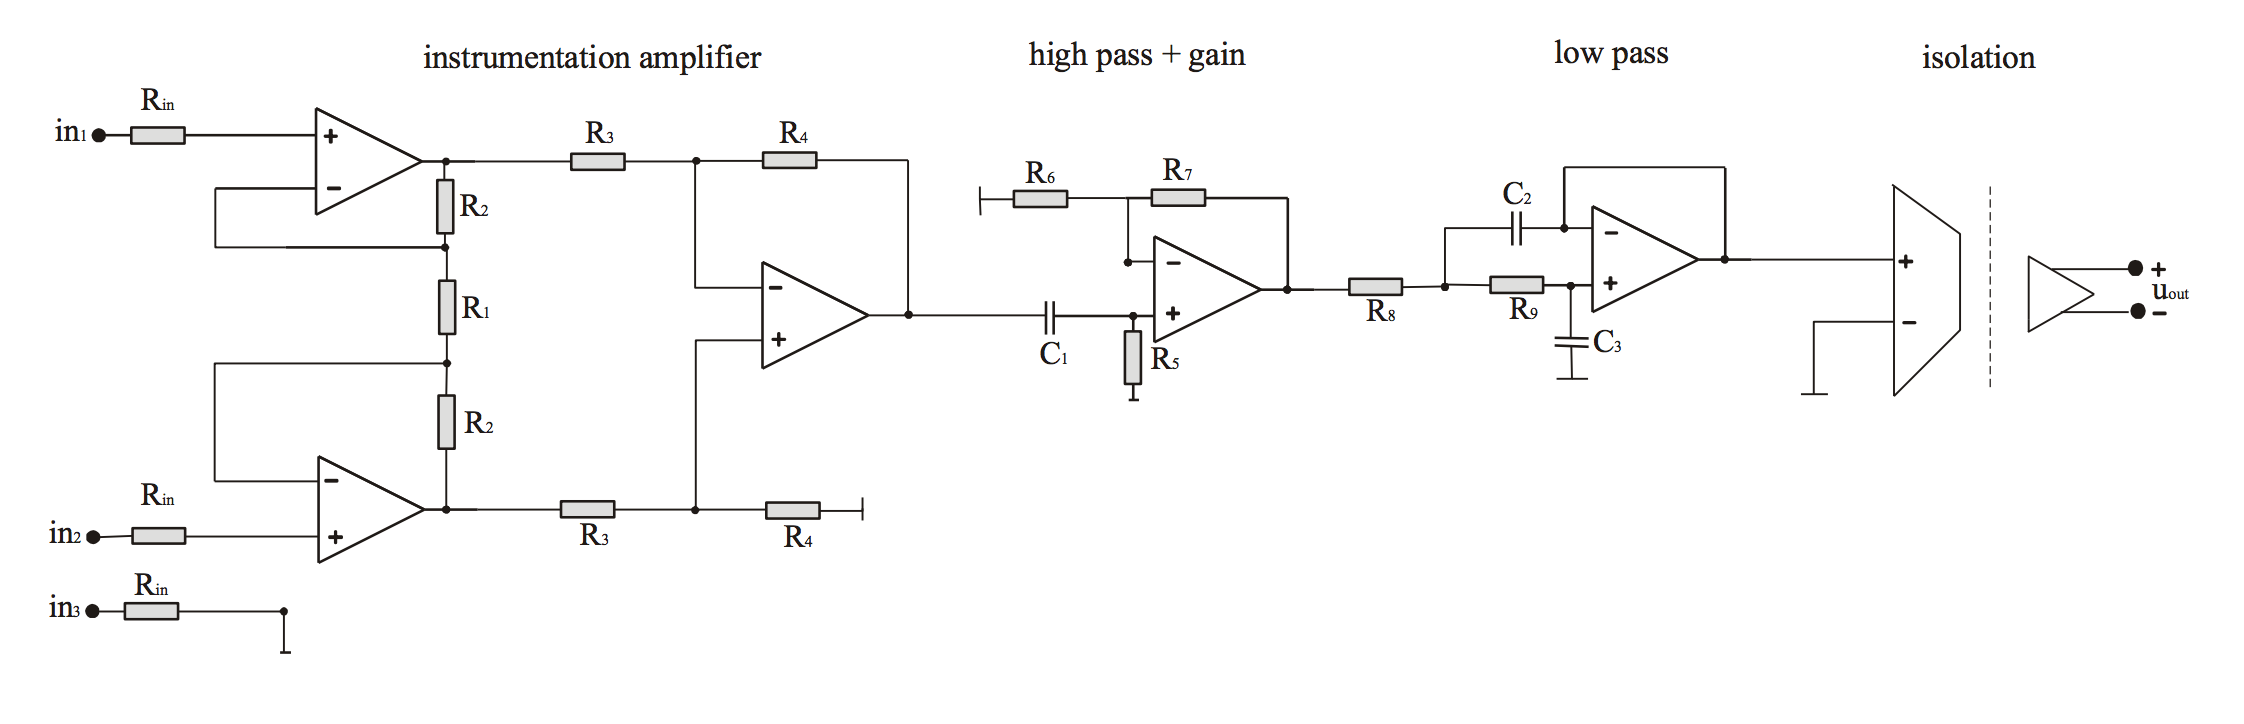
\includegraphics[scale=.35]{ECG_circuit.png}
\caption{Schematic of the circuitry used to amplify ECG signals in the laboratory.}
\label{fig:circuit}
\end{center}
\end{figure}

The first stage of the circuit, the instrumentation amplifier, was designed to have a gain of XX. %did we record this value anywhere or should be take it from the modelsim?
In total, the gain of the ECG amplifier should be 1750. However, it is bad practice to apply all of the gain at a single amplification stage, so for this reason the gain is spread between the three main stages. As Figure \ref{fig:circuit} indicates, the feedback resistors for the voltage followers are equal in value, and related to $R_1$ such that %equation.....

The values of $R_{in}$ should be chosen such that the input impedance of the ECG amplifier circuit is sufficiently high. However, if these values are too large, the 
High input impedance but we use 100k because else the signal disappears

\subsection{AC Analysis}

\begin{figure}[H]
\begin{center}
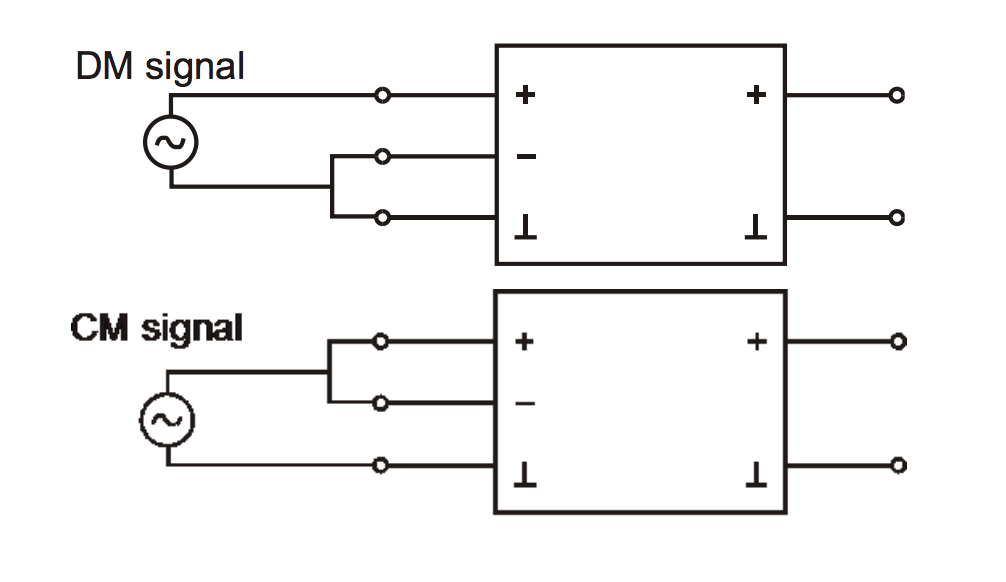
\includegraphics[scale=.5]{DM_CM.png}
\caption{Schematic of the input configurations for measuring DM and CM signals.}
\label{fig:DM_CM}
\end{center}
\end{figure}

\begin{figure}[H]
\begin{center}
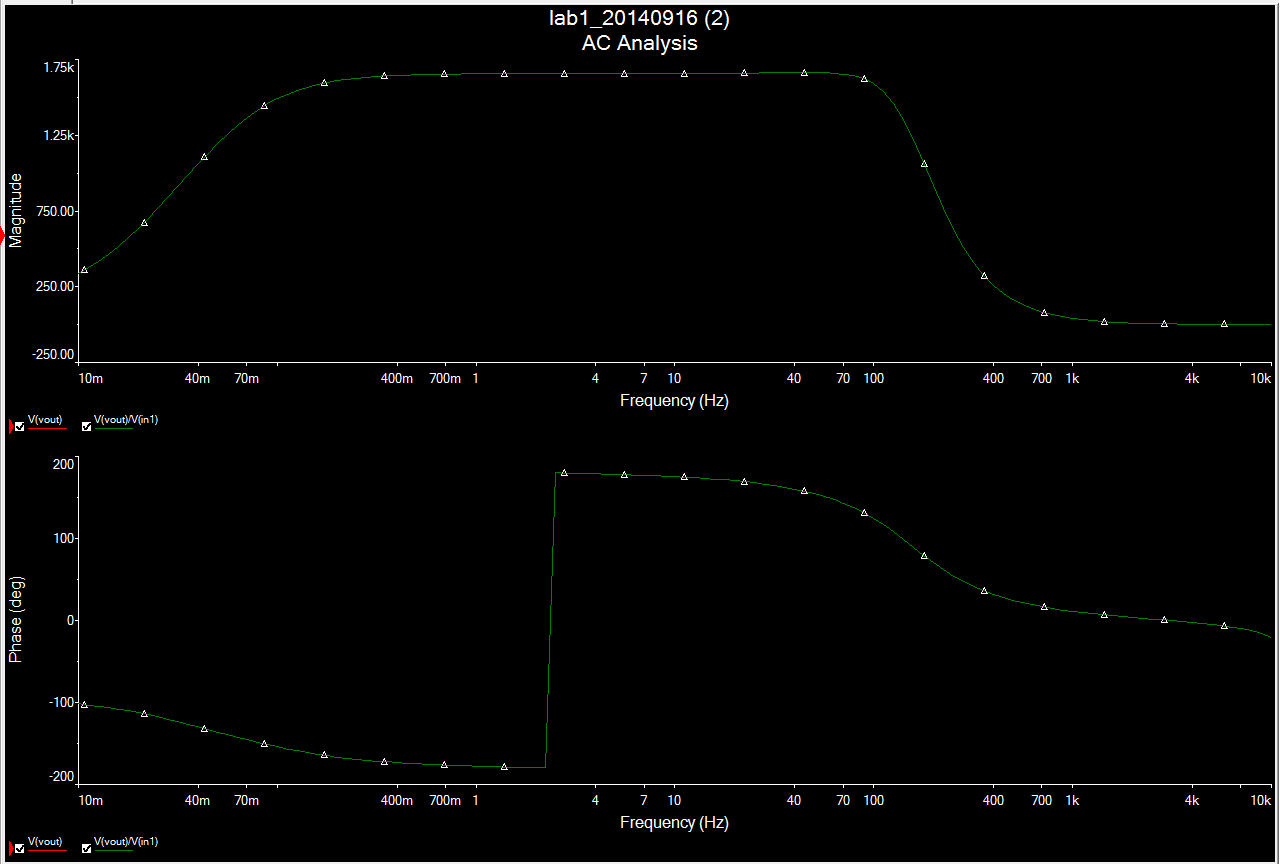
\includegraphics[scale=.35]{DM_analysis.png}
\caption{AC analysis of the simulated ECG amplifier circuit in DM measurement configuration.}
\label{fig:DM}
\end{center}
\end{figure}

\begin{figure}[H]
\begin{center}
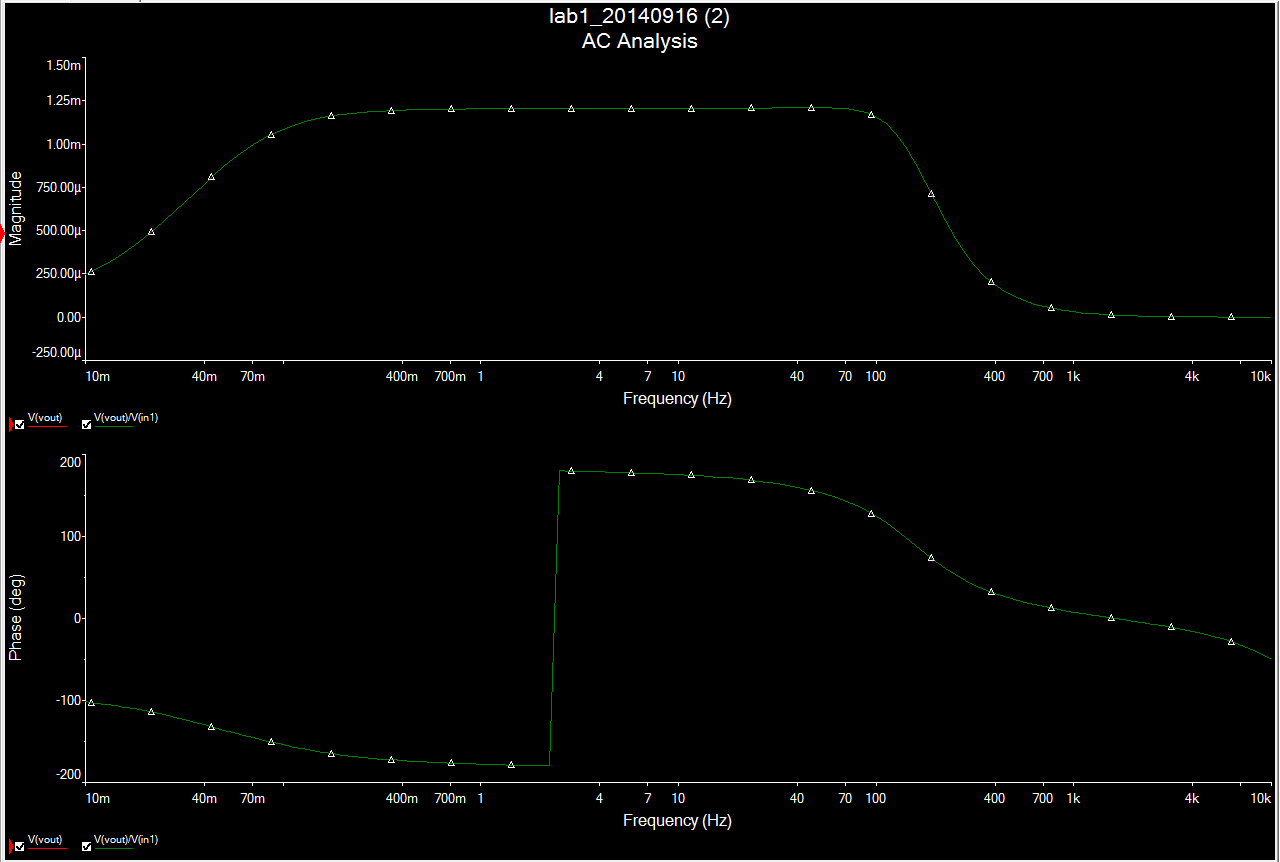
\includegraphics[scale=.35]{CM_analysis.png}
\caption{AC analysis of the simulated ECG amplifier circuit in CM measurement configuration.}
\label{fig:CM}
\end{center}
\end{figure}

\begin{figure}[H]
\begin{center}
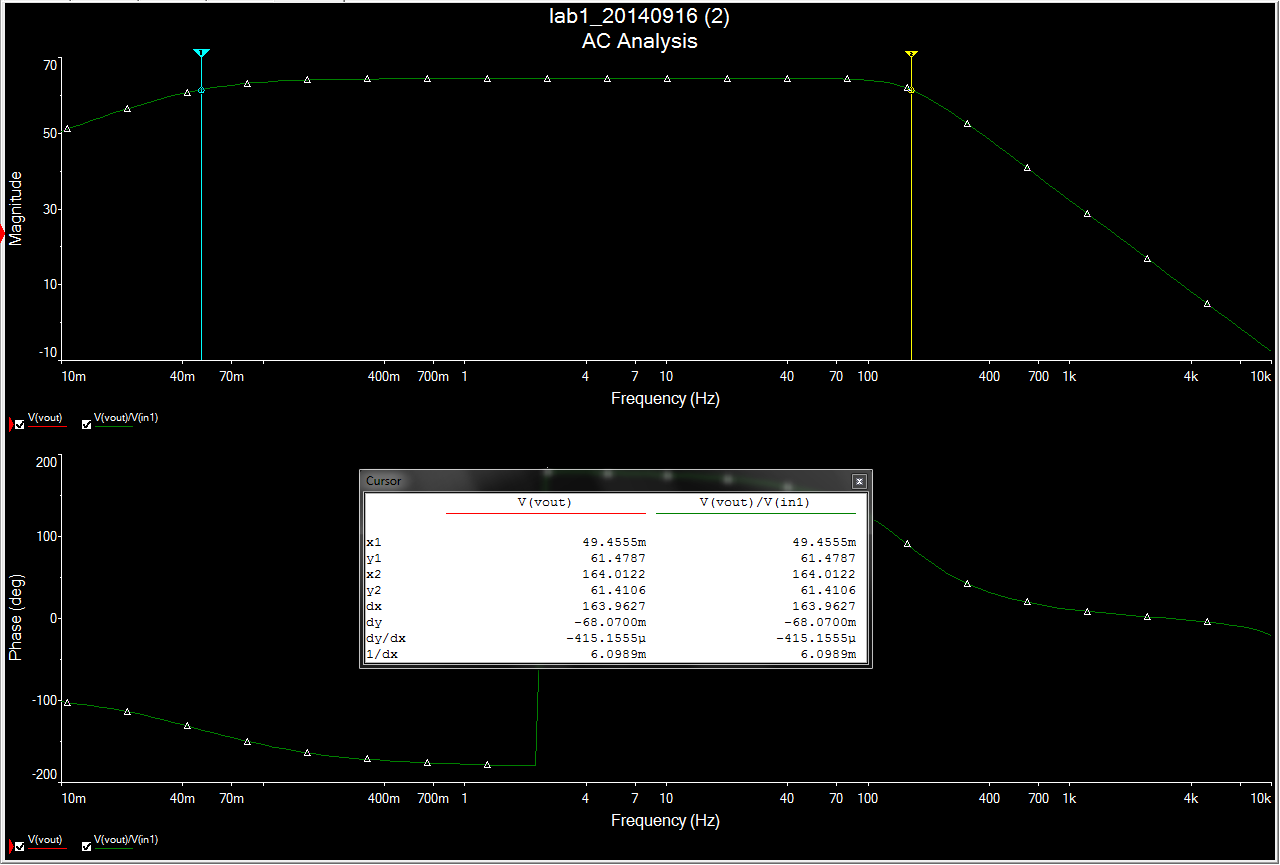
\includegraphics[scale=.35]{3db_analysis.png}
\caption{AC analysis of the simulated ECG amplifier circuit in CM measurement configuration. The y-axis is plotted in decibels in order to easily find the -3dB cutoff frequencies.}
\label{fig:3DB}
\end{center}
\end{figure}

\section{Construction and Data Acquisition}

\begin{figure}[H]
\begin{center}
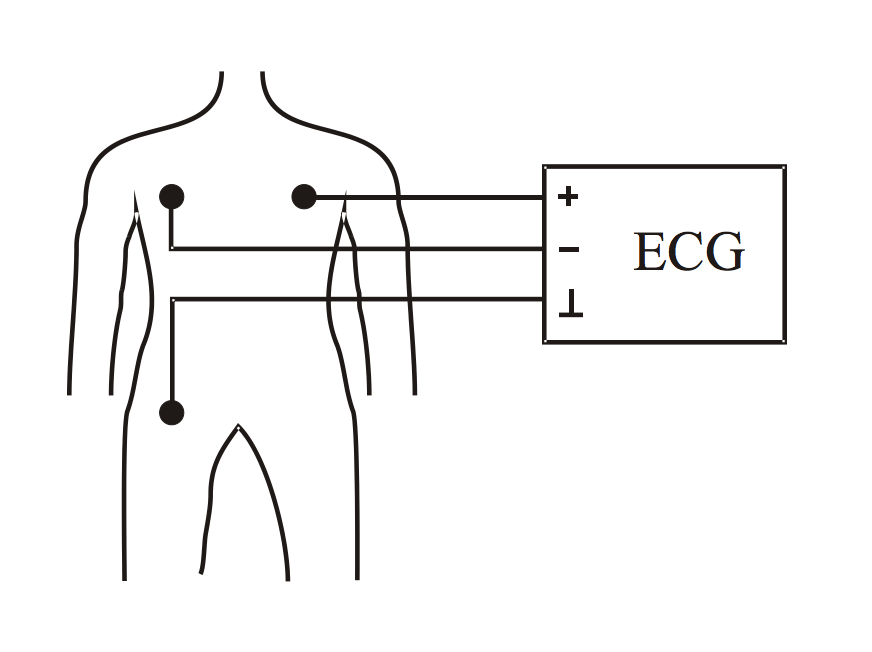
\includegraphics[scale=.5]{setup.png}
\caption{Schematic of the electrode placement for the acquisition of ECG signals in the laboratory.}
\label{fig:setup}
\end{center}
\end{figure}

\section{Results}

\begin{figure}[H]
\begin{center}
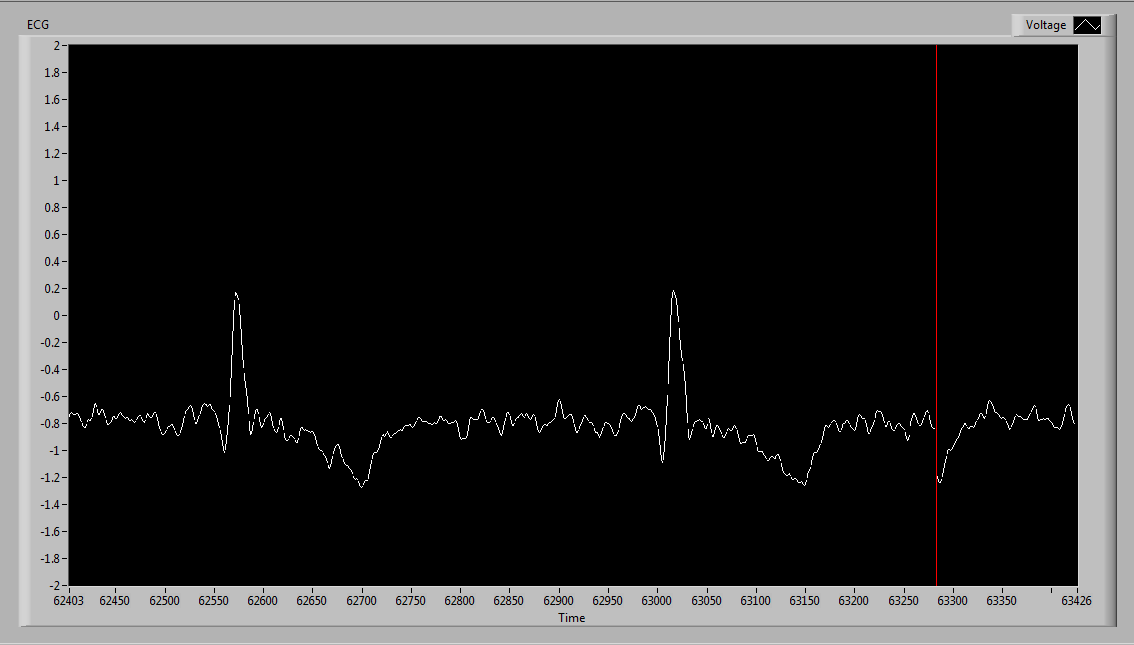
\includegraphics[scale=.4]{ECG_real.png}
\caption{Captured waveform from the ECG amplifier circuit when hooked up to electrodes placed on a patient.}
\label{fig:ECG}
\end{center}
\end{figure}

\section{Device Limitations}

Motion artifact
Using more electrodes for a better picture of heart's activity
Can't see the whole pqrst complex here, can only figure out BPM from the peaks

\begin{thebibliography}{1}

\bibitem{webster}
Webster, John G. Medical Instrumentation Application and Design, 4th Edition. John Wiley \& Sons, 092008. VitalBook file.

\end{thebibliography}

\end{document}